\begin{figure}[h!]
    \centering
    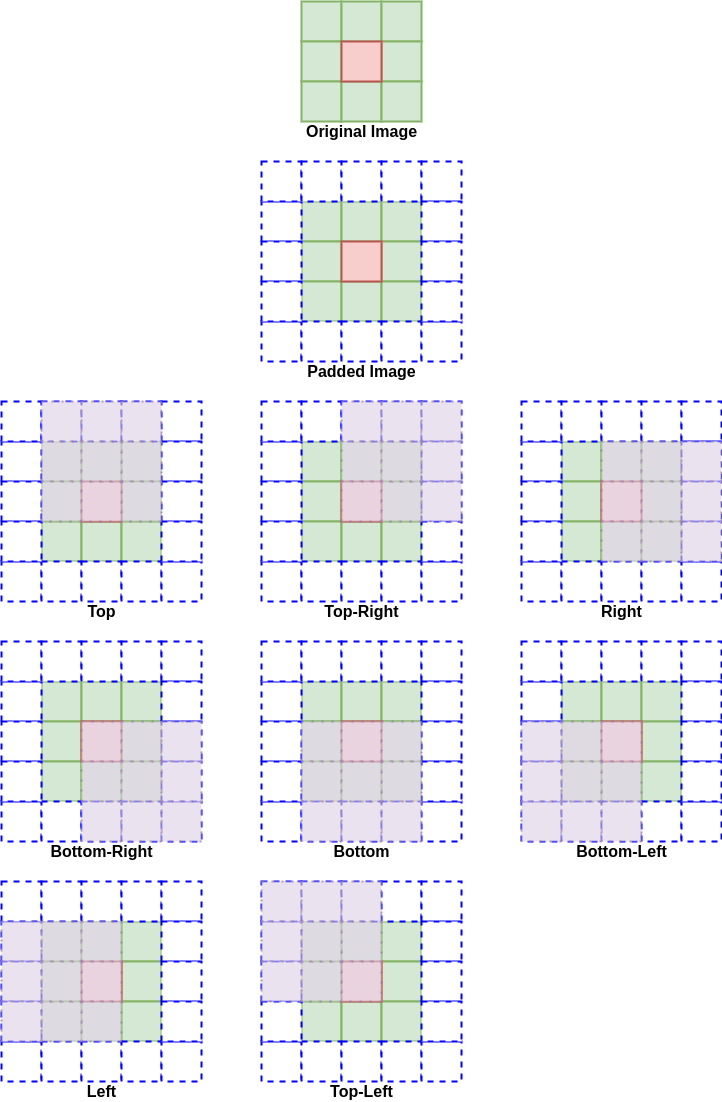
\includegraphics[width=0.4\textwidth]{images/lbp.png}
    \caption{Illustration of our vectorized implementation of LBP texture descriptor.}
    \label{fig:lbp-implementation}
\end{figure}

The feature extraction module includes \textbf{local binary pattern} \emph{(LBP)} texture descriptor. Other feature extractor were considered, as well. However, after many experiments, we found out \emph{LBP} texture descriptor performs the best in our case. The other feature extractors are discussed in later sections. Although \emph{LBP} features offer high accuracy, \textbf{skimage} implementation is not vectorized and heavily depends on \emph{loops}. The extraction of \emph{LBP} features for a single form can take up to $0.5$ second. That's why, we come up with a vectorized implementation that speeds up processing to up to $0.02$ second per form. \\

Figure \ref{fig:lbp-implementation} shows the \textbf{vectorized implementation} on a simple $3X3$ image matrix. The implementation goes as follows :
\begin{enumerate}
    \item The input image is \emph{padded} with \emph{zeros} from all directions with the \emph{LBP} radius size.
    \item An \emph{LBP} map with the same dimensions as the input image is initialized with zeros.
    \item The whole original image is displaced to the top and compared to the padded image. Using this method, we compare all pixels in parallel instead of looping over each pixel.
    \item The resultant map is, then, multiplied by $2$ raised to the power of \emph{number of iteration}, then added to the \emph{LBP} map. \textbf{Note that,} \emph{number of iteration} ranges from $0$ to $7$, as only $8$ directions are considered to speed up the implementation.
    \item Steps $3$ and $4$ are repeated for \emph{top-right}, \emph{right}, \emph{bottom-right}, \emph{bottom}, \emph{bottom-left}, \emph{left} and \emph{top-left} directions.
    \item A histogram is calculated for the output \emph{LBP} map with $256$ bins. The histogram is normalized by its mean, according to the original \emph{LBP} implementation.
\end{enumerate}
